\chapter{Local Features - Scale Invariant Feature Transform}

\noindent
El detector de esquinas de Harris presenta una limitación crítica: \textbf{no es invariante a los cambios de escala}. Un punto que se comporta como una esquina a escala fina se convierte en un borde o una región plana cuando se examina a una escala macroscópica (zoom). \\

\noindent
Para resolver esto, necesitamos detectar estructuras que sean estables en un espacio continuo de posiciones y escalas. El algoritmo \textbf{SIFT (Scale Invariant Feature Transform)} aborda este problema mediante la construcción de un \textit{Scale-Space} (Espacio de Escala).


\section{El Pipeline Completo de SIFT}
El algoritmo SIFT funciona tanto como un \textbf{detector} como un \textbf{descriptor} de características locales a través de 4 pasos estrictos y secuenciales que debes memorizar. \\

\noindent
El objetivo absoluto de SIFT (Scale Invariant Feature Transform) es extraer puntos clave de una imagen que sean tan únicos e invariantes que el ordenador pueda volver a encontrarlos y emparejarlos en otra foto, incluso si esa otra foto ha cambiado de escala (zoom), ha rotado, o tiene una iluminación diferente. \\

\noindent
Básicamente, busca crear un ``DNI matemático'' para partes de la imagen que sea inmune a los cambios del mundo físico.

\subsection{Paso 1: Construcción del Espacio de Escala y Diferencia de Gaussianas (DoG)}
\noindent
Para buscar características en múltiples escalas simultáneamente, la imagen se filtra repetidamente con núcleos Gaussianos utilizando diferentes desviaciones estándar ($\sigma$). 

\begin{itemize}
    \item \textbf{Espacio de Escala $L(x,y,\sigma)$:} se obtiene mediante la convolución de la imagen de entrada $I(x,y)$ con un filtro Gaussiano variable $G(x,y,\sigma)$:
    $$L(x,y,\sigma) = G(x,y,\sigma) * I(x,y)$$
    Las imágenes se organizan en \textbf{Octavas}. Al pasar a la siguiente octava, la imagen se submuestrea a la mitad de su tamaño físico y el valor de $\sigma$ se duplica. \\

    \begin{observacion}
        Una octava no es una sola imagen, sino un grupo o conjunto de imágenes que tienen el mismo tamaño de píxeles, pero diferentes niveles de blur (distinto valor de $\sigma$), por lo que en lo que llamabamos pirámide de escala, cada octava es un bloque vertical de imágenes con misma cantidad de píxeles pero diferentes $\sigma$. \\
        \noindent
        Como todas las imágenes de esta octava mantienen el mismo tamaño (mismos píxeles de ancho y alto), el ordenador puede restarlas directamente entre sí para obtener las matrices DoG (Diferencia de Gaussianas). 
    \end{observacion}
    
    \item \textbf{Difference of Gaussians (DoG):} calcular el \underline{Laplaciano de Gaussiano} ($\text{LoG}$) de forma directa es computacionalmente costoso. SIFT solventa esto aproximando el $\text{LoG}$ mediante la resta aritmética de dos imágenes adyacentes en la escala, separadas por un factor constante $k$:
    $$DoG(x,y,\sigma) = L(x,y,k\sigma) - L(x,y,\sigma)$$
    \observacion{
        La relación de DoG con el LoG es la siguiente
        $$DoG(x,y,\sigma) \approx (k-1)\sigma^2 \nabla^2 L \quad \text{ donde } \text{LoG}=\sigma \nabla^2 L$$
        lo que significa que la matriz DoG es matemáticamente igual al LoG multiplicado por una constante constante $((k-1)\sigma^2)$. Como en SIFT solo nos interesa buscar los puntos donde la respuesta es máxima (los extremos locales), multiplicar toda la matriz por una constante no cambia la posición de los máximos ni de los mínimos. 
    }
\end{itemize}
\noindent
Podemos ver un ejemplo de la pirámide de escala y las imágenes DoG resultantes en la Figura \ref{fig:sift_pyramid}. \\

\begin{figure}
    \centering
    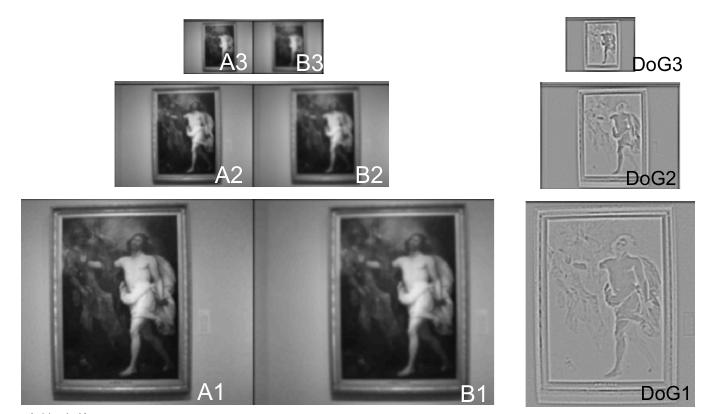
\includegraphics[width=0.8\textwidth]{img/sift_pyramid.png}
    \caption{Ejemplo de pirámide de escala y las imágenes DoG resultantes.}
    \label{fig:sift_pyramid}
\end{figure}

\begin{definicion}[Laplaciano de Gaussiano (LoG)]
    El \tbf{Laplaciano de Gaussiano} es un operador matemático diseñado para detectar estructuras circulares o manchas (llamadas blobs) en una imagen a una escala determinada ($\sigma$). Se compone de dos pasos lógicos combinados en un solo filtro:
    \begin{itemize}
        \item \textbf{Suavizado Gaussiano:} primero se aplica un filtro Gaussiano a la imagen para eliminar el ruido y seleccionar la escala del detalle que queremos buscar (controlada por $\sigma$).
        \item \tbf{Operador Laplaciano ($\nabla^2$):} después se calcula la segunda derivada espacial ($L_{xx} + L_{yy}$). Físicamente, la derivada segunda busca dónde terminan las rampas de brillo. Cuando se aplica sobre una estructura circular que coincide con el tamaño del filtro, la respuesta matemática alcanza un pico máximo (un extremo).
    \end{itemize}
\end{definicion}

\subsection{Paso 2: Keypoint Localization}
\noindent
Una vez obtenidas las matrices DoG, el algoritmo busca candidatos a puntos clave identificando los \textbf{extremos locales} (máximos o mínimos) en un entorno tridimensional (posición y escala):
\begin{itemize}
    \item Cada píxel en una imagen DoG se compara con sus $8$ vecinos espaciales en la misma capa, más los $9$ vecinos de la capa superior y los $9$ vecinos de la capa inferior (un total de $26$ comparaciones). Si el valor del píxel central es estrictamente mayor que los 26 vecinos, o estrictamente menor que los 26 vecinos, se le corona como \tbf{extremo local} (Máximo o Mínimo), y se almacena como sigue
    \begin{equation*}
        \mathbf{x}=\{x,y,\sigma\}
    \end{equation*}
    \item \textbf{Refinamiento y Eliminación de puntos inestables:} muchos candidatos iniciales son inestables. Se aplica una aproximación por serie de Taylor para localizar el extremo con precisión sub-píxel. Se descartan de forma inmediata:
    \begin{enumerate}
        \item Los puntos con bajo contraste (sensibles al ruido).
        \item Los puntos localizados a lo largo de bordes rectos (falsos positivos). Tomamos $H$ la matriz Hessiana de la DoG en el punto clave, y tenemos que si se cumple
        \begin{equation*}
            \dfrac{(\lambda_1 + \lambda_2)^2}{\lambda_1 \lambda_2} > \dfrac{(r+1)^2}{r}
        \end{equation*}
        con $r=10$, entonces el punto se descarta por ser demasiado parecido a un borde (un eigenvalor es mucho mayor que el otro), porque a la hora de intentar emparejarlo con otra imagen, va a coincidir con cualquier borde que tenga la misma orientación, lo que genera muchos falsos positivos.
        
    \end{enumerate}
\end{itemize}

\subsection{Paso 3: Keypoint Orientation Assignment}
\noindent
Para lograr la \textbf{invariancia a la rotación}, se calcula una dirección dominante para cada punto clave superviviente (dada la ubicación $(x,y)$ y la capa $\sigma$) basada en las propiedades del gradiente local:
\begin{itemize}
    \item Se calcula la magnitud $m(x,y)$ y la orientación $\theta(x,y)$ del gradiente en una vecindad Gaussiana alrededor del punto.
    \item Se crea un \tbf{histograma de orientaciones} con 36 contenedores (\textit{bins}), donde cada contenedor cubre un rango de $10^\circ$. Cada píxel vota en el histograma ponderado por la magnitud de su gradiente y por una ventana Gaussiana central.
    \begin{itemize}
        \item El voto de un píxel no vale $1$, vale la magnitud de su propio gradiente (si el brillo cambia mucho, su voto tiene mucha fuerza) multiplicado por una ventana Gaussiana central. Esto significa que los píxeles que están pegados al punto clave tienen votos sumamente importantes, mientras que los píxeles que están más alejados en los bordes de la ventana apenas influyen en el resultado.
    \end{itemize}
    \item El pico más alto del histograma se define como la \textbf{orientación dominante} del punto clave. Si existe otro pico que supere el 80\% del máximo, se crea un segundo punto clave independiente en la misma posición pero con esta nueva orientación.
\end{itemize}

\begin{observacion}
    Es perfectamente posible que coincidan puntos clave en el mismo píxel de la misma octava. Si tienen distinto blur, significa que ese mismo punto del espacio contiene información física de diferentes tamaños (un detalle pequeño y una estructura grande a la vez). Si tienen el mismo blur, puede deberse a que el punto tiene múltiples orientaciones dominantes que superaron el umbral del 80\%.
\end{observacion}

\subsection{Paso 4: Descriptor Generation}
\noindent
Con la posición, escala y orientación fija, el algoritmo construye la firma matemática (descriptor):
\begin{enumerate}
    \item Tomar la imagen suavizada por Gauss a la escala $\sigma$ del punto clave.
    \item Se toma una ventana de $16 \times 16$ píxeles alrededor del punto clave.
    \item La ventana se \textbf{rota alineándola con la orientación dominante} calculada en el paso anterior (garantizando inmunidad al giro). \\
    \noindent
    Esto sirve para que podamos alinear el descriptor con la dirección de la característica, de modo que si la imagen se gira, el descriptor se ajustará automáticamente a esa rotación, manteniendo su consistencia, con la imagen original.
    \item Esta ventana de $16 \times 16$ se subdivide en 16 sub-bloques más pequeños de $4 \times 4$ píxeles cada uno.
    \item Para cada sub-bloque de $4 \times 4$, se calcula un histograma de orientaciones de gradiente abreviado con 8 contenedores (direcciones cardinales principales), donde cada píxel vota con su magnitud de gradiente. Esto da un vector de 8 dimensiones por sub-bloque.
    \item El descriptor final es la concatenación de todos los histogramas
    $$16 \text{ sub-bloques} \times 8 \text{ direcciones} = \mathbf{128 \text{ dimensiones}}$$ 
    un vector de 128 números.
    \item Al final se aplica \tbf{normalización} (inmunidad lumínica): ese vector de 128 números se divide por su norma euclídea ($L_2$). Al normalizar el vector a longitud unidad, si multiplicas el brillo de la imagen entera por dos (un cambio de iluminación global), las magnitudes de los gradientes se duplican, pero al normalizar, el vector final de 128 números vuelve a dar exactamente el mismo resultado. El descriptor se vuelve invariante a la iluminación.
\end{enumerate}



\section{¿Por qué SIFT es Invariante? (Justificación Teórica)}
Memorizar las razones exactas de su robustez frente al mundo físico:
\begin{itemize}
    \item \textbf{Invariancia a la Escala:} gracias a la estructura de \textbf{pirámide multi-escala} y la búsqueda tridimensional de extremos en el espacio DoG (lo que se hace en Paso 2 al trabajar con la posición $(x,y)$ y la escala $\sigma$). La característica se detectará en la capa que mejor se adapte a su tamaño real.
    \item \textbf{Invariancia a la Rotación:} gracias a la \textbf{asignación de la orientación dominante}. Como el descriptor rota sus ejes adaptándose a este ángulo antes de medir los gradientes, la firma de 128 dimensiones no cambia si la imagen se gira.
    \item \textbf{Invariancia a la Iluminación:} al basarse puramente en gradientes de intensidad (derivadas métricas), se eliminan los desplazamientos constantes de brillo. Además, el vector final de 128 dimensiones se \textbf{normaliza a longitud unidad} ($L_2$), lo que cancela los cambios multiplicativos de contraste.
\end{itemize}

\subsection{Limitaciones de SIFT}
\begin{itemize}
    \item \tbf{Lento y costoso computacionalmente}: la construcción de decenas de niveles Gaussianos, restas DoG e histogramas densos de 128 dimensiones consume demasiados recursos, imposibilitando su uso nativo en sistemas de tiempo real embebidos o robótica ligera antigua.
\end{itemize}


\section{Evolución y Alternativas: SURF, BRIEF y ORB}
Debido a la lentitud de SIFT, surgieron variantes optimizadas en la literatura:

\subsection{SURF (Speeded Up Robust Features)}
\noindent
SURF nace con una sola misión: replicar la robustez de SIFT a la escala y la rotación, pero reduciendo drásticamente el tiempo de cálculo.
\begin{itemize}
    \item \textbf{Filosofía:} es una versión acelerada de SIFT basada en aproximaciones drásticas, usando \tbf{filtros de caja cuadrados} (Box Filters) ($\mathcal{O}(1)$) en lugar de Gaussianos (no hacemos tantas multiplicaciones de flotantes), y aprovechando las \textbf{imágenes integrales} para calcular respuestas de escala en tiempo constante ($\mathcal{O}(1)$).
    \item \textbf{Detection}: utiliza un detector basado en la matriz Hessiana, donde el Laplaciano se aproxima con filtros de caja de $9 \times 9$ aplicados sobre la imagen integral. 
    \item \textbf{Scale-space}: en lugar de reducir la imagen, SURF aumenta el tamaño del filtro para simular la búsqueda en escala, evitando el submuestreo (empezamos con un filtro de $9 \times 9$, luego pasamos a uno de $15 \times 15$, $21 \times 21$, etc.). Como la imagen integral tarda lo mismo en procesar un filtro pequeño que uno gigante, escalar el filtro es gratis a nivel computacional.
    \item \textbf{Resultado:} mucho más rápido que SIFT, aunque a veces sacrifica precisión en transformaciones de perspectiva extremas. Su descriptor estándar se reduce a 64 dimensiones.
\end{itemize}
\begin{observacion}
    $I_{\sum}(x,y)=\sum_{i=0}^{x}\sum_{j=0}^{y}I(i,j)$ es la imagen integral, que permite calcular la suma de cualquier región rectangular en tiempo constante con solo 4 accesos a memoria.
\end{observacion}

\subsection{BRIEF vs ORB: Descriptores Binarios}
\noindent
Para entornos de tiempo real estricto, la distancia Euclídea entre vectores flotantes (como las 128 dimensiones de SIFT) es un cuello de botella. Nacen los descriptores binarios:

\begin{itemize}
    \item \textbf{BRIEF (Binary Robust Independent Elementary Features):}
    \begin{itemize}
        \item \textbf{Concepto:} no calcula histogramas ni gradientes. Toma un parche suavizado y realiza una serie de \underline{pruebas de comparación binarias de intensidad} (brillo) entre parejas de píxeles aleatorias predefinidas.
        \item \textbf{El código:} Si el píxel $A > B \rightarrow 1$; si no $\rightarrow 0$, es decir
        $$\tau(p; A, B) = \begin{cases} 1 & \text{si } I(A) > I(B) \\ 0 & \text{si } I(A) \le I(B) \end{cases}$$
        y se tiene que el descriptor es una cadena de bits (ej. 256 bits). El matching es ultra veloz porque se mide con la \tbf{distancia de Hamming} (operaciones XOR a nivel de procesador).
        \item \textbf{Defecto crítico:} \textit{¡Pregunta típica de examen!} BRIEF **NO es invariante a la rotación**. Si la imagen gira, las parejas fijas de píxeles apuntan a zonas erróneas.
    \end{itemize}
    
    \item \textbf{ORB (Oriented FAST and Rotated BRIEF):}
    \begin{itemize}
        \item \textbf{Concepto:} es la alternativa moderna, libre de patentes y ultra eficiente para tiempo real.
        \item \textbf{Mejora sobre BRIEF:} añade invariancia a la rotación calculando el \textbf{centroide de intensidad} del parche para deducir su orientación. Luego, rota de forma solidaria el patrón de pruebas binarias de BRIEF antes de generar la cadena de bits. \\
        
        \noindent
        El algoritmo calcula el centroide de intensidad (el ``centro de masa'' del brillo) del parche. Imagina que el parche es una superficie y el brillo es el peso. Si un lado del parche es muy blanco y brillante, y el otro es oscuro, el centro de masa se desplazará hacia la zona brillante. ORB traza un vector que va desde el centro geométrico del parche $(0,0)$ hasta ese centroide de intensidad $(C_x, C_y)$. El ángulo de este vector se convierte en la orientación del punto clave ($\theta$).

        \item \textbf{Ventajas:} es tan rápido como BRIEF, inmune a la rotación, y órdenes de magnitud más veloz que SIFT, ideal para SLAM visual en tiempo real.
    \end{itemize}
\end{itemize}

